

\documentclass[a4paper,11pt]{report}
\usepackage[showexo=true,showcorr=false,showdegree=true]{../packages/coursclassed}
%Commenter ou enlever le commentaire sur la ligne suivante pour montrer le niveau
\toggletrue{montrerNiveaux}
%permet de gérer l'espacement entre les items des env enumerate et enumitem
\usepackage{enumitem}
\setlist[enumerate]{align=left,leftmargin=1cm,itemsep=10pt,parsep=0pt,topsep=0pt,rightmargin=0.5cm}
\setlist[itemize]{align=left,labelsep=1em,leftmargin=*,itemsep=0pt,parsep=0pt,topsep=0pt,rightmargin=0cm}
%permet de gerer l'espacement entre les colonnes de multicols
\setlength\columnsep{35pt}
\usepackage{tikz}

\newcount\segmentsleft
\tikzset{pics/.cd,
  circle fraction/.style args={#1/#2}{code={%
\segmentsleft=#1\relax
\pgfmathloop
\ifnum\segmentsleft<1\else
\ifnum\segmentsleft<#2 \edef\n{\the\segmentsleft}\else\def\n{#2}\fi
\begin{scope}[shift={(\pgfmathcounter,0)}]
\foreach \i [evaluate={\a=360/#2*(\i-1)+90;}] in {1,...,\n}
  \fill[fill=gray!70] (0,0) -- (\a:3/8) arc (\a:\a+360/#2:3/8) -- cycle;
\draw circle [radius=3/8];
\ifnum#2>1
  \foreach \i [evaluate={\a=360/#2*(\i-1);}] in {1,...,#2}
    \draw (0,0) -- (90+\a:3/8);
\fi
\end{scope}
\advance\segmentsleft by-#2
\repeatpgfmathloop
  }}
}


\newcommand{\vfracrect}[3][]{\tikz[rotate=270,baseline, #1]{
    \foreach \n in {1,...,#2}{\draw[thick, fill=gray!70] ({(\n-1)/#3},0) rectangle (\n/#3,1);}
    \foreach \n in {#2,...,#3} {\draw[thick] ({(\n-1)/#3},0) rectangle (\n/#3,1);}}}

    \newcommand{\vemptyfracrect}[2][]{\tikz[rotate=270,baseline, #1]{
    \foreach \n in {1,...,1}{\draw[thick] ({(\n-1)/#2},0) rectangle (\n/#2,1);}
    \foreach \n in {1,...,#2} {\draw[thick] ({(\n-1)/#2},0) rectangle (\n/#2,1);}}}

\newcommand{\fracrect}[3][]{\tikz[baseline, #1]{
    \foreach \n in {1,...,#2}{\draw[thick, fill=gray!70] ({(\n-1)/#3},0) rectangle (\n/#3,1);}
    \foreach \n in {#2,...,#3} {\draw[thick] ({(\n-1)/#3},0) rectangle (\n/#3,1);}}}

    \newcommand{\emptyfracrect}[2][]{\tikz[baseline, #1]{
    \foreach \n in {1,...,1}{\draw[thick] ({(\n-1)/#2},0) rectangle (\n/#2,1);}
    \foreach \n in {1,...,#2} {\draw[thick] ({(\n-1)/#2},0) rectangle (\n/#2,1);}}}



\newcommand{\emptyfrac}[1][]{\tikz[baseline=-.6ex,#1]{\draw (0,0)--
    node[above=1pt, fill=gray!20, minimum size=7mm]{}
    node[below=1pt, fill=gray!20, minimum size=7mm]{}(.5,0);}}

    
\makeatletter
\renewcommand*\env@matrix[1][\arraystretch]{%
  \edef\arraystretch{#1}%
  \hskip -\arraycolsep
  \let\@ifnextchar\new@ifnextchar
  \array{*\c@MaxMatrixCols c}}
\makeatother

\begin{document}

%%%%%%%%%%%%%%%%% À MODIFIER POUR CHAQUE SERIE %%%%%%%%%%%%%%%%%%%%%%%%%%%%%
\newcommand{\chapterName}{Nombres et opérations}
\newcommand{\serieName}{Les fractions}

%%%%%%%%%%%%%%%%%% PREMIERE PAGE NE PAS MODIFER %%%%%%%%%%%%%%%%%%%%%%%%
% le chapitre en cours, ne pas changer au cours d'une série
\chapter*{\chapterName}
\thispagestyle{empty}

\begin{amL}{\serieName}{
\item Nombres rationnels (page 27)
\item Passer d'une écriture décimale finie à une écriture fractionnaire (page 28)
\item Amplification et simplification de fractions (page 29)
\item Addition et soustraction de fractions (page 30)
}
\end{amL}
\section*{\serieName}
\setcounter{page}{1}





%%%%%%%%%%%%%%% EXERCICES %%%%%%%%%%%%%%%%%%%%%%%%%%%%%


\begin{QSJ}{30}{1}
\end{QSJ}

%représentation

\begin{exof}{NO98}{33}{1}
\end{exof}
\begin{exof}{NO97}{32}{1}
\end{exof}

\begin{exop}{
	Détermine à quelle fraction correspond chacune des parties grisées.
		\begin{tasks}(3)
		\task 

			\scalebox{2.5}{
		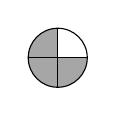
\begin{tikzpicture}
  %\node at (-1/2,0) {$\ldots\ldots\ldots$};
  \pic  at (0, 0) {circle fraction={3/4}};
\end{tikzpicture}}

\hrulefill
		\task 

			\scalebox{2.5}{
		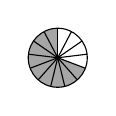
\begin{tikzpicture}
  %\node at (-1/2,0) {$\ldots\ldots\ldots$};
  \pic  at (0, 0) {circle fraction={9/13}};
\end{tikzpicture}}

\hrulefill
		\task 

			\scalebox{2.5}{
		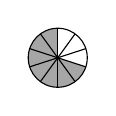
\begin{tikzpicture}
  %\node at (-1/2,0) {$\ldots\ldots\ldots$};
  \pic  at (0, 0) {circle fraction={7/10}};
\end{tikzpicture}}

\hrulefill
		\task 

			\scalebox{2.5}{
				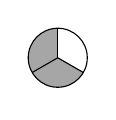
\begin{tikzpicture}
  %\node at (-1/2,0) {$\ldots\ldots\ldots$};
  \pic  at (0, 0) {circle fraction={2/3}};
\end{tikzpicture}}

\hrulefill
		\task 

			\scalebox{2.5}{
				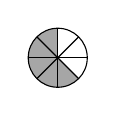
\begin{tikzpicture}
  %\node at (-1/2,0) {$\ldots\ldots\ldots$};
  \pic  at (0, 0) {circle fraction={5/8}};
\end{tikzpicture}}

\smallskip

\hrulefill

		\task

			\scalebox{2.5}{
				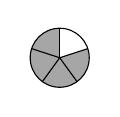
\begin{tikzpicture}
  %\node at (-1/2,0) {$\ldots\ldots\ldots$};
  \pic  at (0, 0) {circle fraction={4/5}};
\end{tikzpicture}}


\vspace{2pt} 

\hrulefill
\end{tasks}
}{1}\end{exop}


\begin{exop}{
	Détermine à quelle fraction correspond chacune des parties grisées.
		\begin{tasks}(2)
		\task 

			\scalebox{2.5}{
		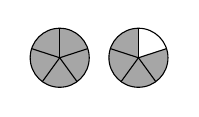
\begin{tikzpicture}
  %\node at (-1/2,0) {$\ldots\ldots\ldots$};
  \pic  at (0, 0) {circle fraction={9/5}};
\end{tikzpicture}}

\hrulefill

		\task 


			\scalebox{2.5}{
		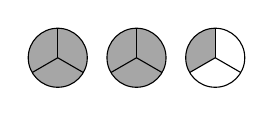
\begin{tikzpicture}
  %\node at (-1/2,0) {$\ldots\ldots\ldots$};
  \pic  at (0, 0) {circle fraction={7/3}};
\end{tikzpicture}}

\hrulefill
		\task 

			\scalebox{2.5}{
		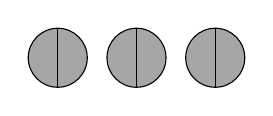
\begin{tikzpicture}
  %\node at (-1/2,0) {$\ldots\ldots\ldots$};
  \pic  at (0, 0) {circle fraction={6/2}};
\end{tikzpicture}}

\hrulefill
		\task 

			\scalebox{2.5}{
				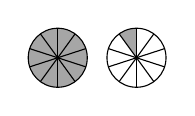
\begin{tikzpicture}
  %\node at (-1/2,0) {$\ldots\ldots\ldots$};
  \pic  at (0, 0) {circle fraction={11/10}};
\end{tikzpicture}}

\hrulefill
		\task 

			\scalebox{2.5}{
				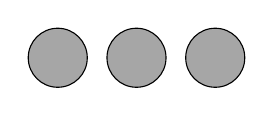
\begin{tikzpicture}
  %\node at (-1/2,0) {$\ldots\ldots\ldots$};
  \pic  at (0, 0) {circle fraction={3/1}};
\end{tikzpicture}}

\hrulefill
		\task 

			\scalebox{2.5}{
				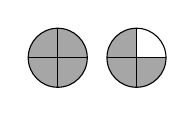
\begin{tikzpicture}
  %\node at (-1/2,0) {$\ldots\ldots\ldots$};
  \pic  at (0, 0) {circle fraction={7/4}};
\end{tikzpicture}}

\hrulefill
	\end{tasks}
}{1}\end{exop}

\begin{exop}{
	Détermine la fraction représentée par les parties grisées.
	\begin{tasks}(2)
		\task 
			
			$\fracrect[xscale=4]{3}{4}$

			\hrulefill

		\task 
			
			$\fracrect[xscale=4]{5}{8}$

\hrulefill

		\task 
			
			$\fracrect[xscale=4]{6}{6}$	
			\vspace{2pt}

		\hspace{24pt}$\fracrect[xscale=4]{4}{6}$

\hrulefill

		\task 
			
			$\fracrect[xscale=4]{7}{11}$

\hrulefill

		\task 
			
			$\fracrect[xscale=4]{3}{10}$

\hrulefill

		\task 
			
			$\emptyfracrect[xscale=4]{9}$

\hrulefill

\vspace{1cm}
\phantom{test}

	\end{tasks}
}{1}\end{exop}

\begin{exof}{NO108}{36}{1}
\end{exof}
\begin{exof}{NO111}{38}{2}
\end{exof}

\begin{resolu}{De la fraction décimale à l'écriture décimale}
{Détermine le nombre décimal correspondant aux fractions suivantes.

{\color{blue} Afin de déterminer l'écriture décimale d'une fraction décimale, il faut déplacer la virgule du numérateur vers la gauche autant de fois qu'il y a de zéros dans le dénominateur.}

\begin{tasks}(2)
    \task $\dfrac{3}{100}={{\color{blue}=0,03 }}$
    \task $\dfrac{5}{10}={{\color{blue}=0,5}}$
    \task $\dfrac{10}{10}={{\color{blue}=1}}$
    \task $\dfrac{8}{1000}={{\color{blue}=0,008}}$
\end{tasks}
 \vspace{1pt}
}{1}
\end{resolu}

\begin{exo}{
	Détermine le nombre décimal correspondant aux fractions suivantes.
	\begin{tasks}(3)
		\task $\dfrac{370}{10}$
		\task $\dfrac{91}{1000}$
		\task $\dfrac{218}{10000}$
		\task $\dfrac{111}{10}$
		\task $\dfrac{2020}{10}$
		\task $\dfrac{35311}{100000}$
	\end{tasks}
 \vspace{1pt}
}{1}\end{exo}


\begin{exo}{
	Détermine la fraction décimale correspondant aux nombres suivants.
	\begin{tasks}[after-item-skip=0.2em, after-skip=-0.5em](3)
		\task $0,13$
		\task $0,4$
		\task $0,752$
		\task $0,5353$
		\task $0,14$
		\task $0,33$
	\end{tasks}
 \vspace{1pt}
}{1}\end{exo}


\begin{exo}{
	Détermine la fraction décimale correspondant aux nombres suivants.
	\begin{tasks}[after-item-skip=0.2em](3)
		\task $7,942$
		\task $1,32$
		\task $11,7$
		\task $980,01$
		\task $97,361$
		\task $0,920101$
	\end{tasks}
 \vspace{1pt}
}{2}\end{exo}

\begin{resolu}{De l'écriture fractionnaire à décimale}
{Écris les nombres suivants sous forme décimale.

{\color{blue} Afin de déterminer l'écriture décimale d'une fraction, il faut calculer le quotient du numérateur par le dénominateur.}

\begin{tasks}(2)
    \task $\dfrac{3}{4}={{\color{blue}3\div 4=0,75}}$
    \task $\dfrac{5}{10}={{\color{blue}5\div 10=0,5}}$
    \task $\dfrac{10}{8}={{\color{blue}10\div 8=1,25}}$
    \task $\dfrac{8}{5}={{\color{blue}8\div 5=1,6}}$
\end{tasks}
 \vspace{1pt}
}{1}
\end{resolu}

\begin{exop}{
Écris les nombres suivants sous forme décimale.
\begin{tasks}(2)
	\task $\dfrac{4}{5}=\hrulefill$\hspace{0.5cm}
    \task $\dfrac{30}{25}=\hrulefill$
    \task $\dfrac{1}{2}=\hrulefill$\hspace{0.5cm}
    \task $\dfrac{8}{10}=\hrulefill$
    \task $\dfrac{3}{15}=\hrulefill$\hspace{0.5cm}
    \task $\dfrac{8}{5}=\hrulefill$
\end{tasks}
 \vspace{1pt}

}{1}\end{exop}

\begin{exo}{
Écris les nombres suivants dans leur forme périodique.
\begin{tasks}(2)
    \task $\dfrac{2}{3}=\hrulefill$\hspace{0.5cm}
    \task $\dfrac{2}{9}=\hrulefill$
    \task $\dfrac{7}{11}=\hrulefill$\hspace{0.5cm}
    \task $\dfrac{5}{9}=\hrulefill$
\end{tasks}
 \vspace{1pt}

}{2}\end{exo}

\begin{exo}{
Écris les nombres suivants sous forme décimale ou périodique.
\begin{tasks}(2)
    \task $\dfrac{1}{3}=\hrulefill$\hspace{0.5cm}
    \task $\dfrac{5}{2}=\hrulefill$
    \task $\dfrac{6}{100}=\hrulefill$\hspace{0.5cm}
    \task $\dfrac{10}{4}=\hrulefill$
    \task $\dfrac{8}{9}=\hrulefill$\hspace{0.5cm}
    \task $\dfrac{9}{7}=\hrulefill$
\end{tasks}
 \vspace{1pt}

}{2}\end{exo}


\begin{exop}{
Détermine l'écriture décimale des nombres suivants.
\begin{tasks}(2)
    \task $\dfrac{7}{3}=\hrulefill$\hspace{0.5cm}
    \task $\dfrac{8}{9}=\hrulefill$
    \task $\dfrac{4}{11}=\hrulefill$\hspace{0.5cm}
    \task $\dfrac{11}{15}=\hrulefill$
    \task $\dfrac{19}{33}=\hrulefill$\hspace{0.5cm}
    \task $\dfrac{3}{7}=\hrulefill$
\end{tasks}
 \vspace{1pt}

}{2}\end{exop}

\begin{exof}{NO99}{33}{1}
\end{exof}

\begin{resolu}{Placer des fractions sur une droite}{
Dessine une droite numérique (entre -4 et 9) et places-y le plus précisément possible les nombres suivants.

{\color{blue} On écrit la fraction sous forme décimale avec une précision qui dépend de la graduation, puis on place le nombre sur la droite. 
}

\begin{tasks}(1)
	\task $-\dfrac{24}{5}=-24\div 5=-4,8$
	\task $\dfrac{31}{4}=31\div 4=7,75\simeq 7,8$
	\task $-\dfrac{1}{6}=-1\div 6\simeq -0,1\overline{6}$
\end{tasks}
\centering
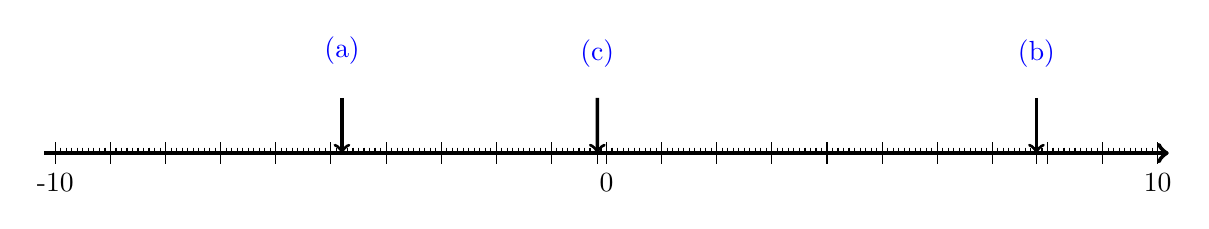
\begin{tikzpicture}[scale=0.7]
  \draw[->,ultra thick] (-10.2,0) -- (10.2,0);
  \foreach \i in {-10,-9,...,10} % numbers on line
    \draw ({10*\i/10},0.2) -- + (0,-0.4) node[below] {}; % tick and their labels
  \draw ({10*(-10)/10},0.2) -- + (0,-0.4) node[below] {-10};
  \draw (0,0.2) -- + (0,-0.4) node[below] {0};
  \draw ({10*(10)/10},0.2) -- + (0,-0.4) node[below] {10};
  \foreach \i in {-100,-99,...,100} % numbers on line
    \draw ({10*\i/100},0.1) -- + (0,-0.1) node[below] {}; % tick and their labels

  % réponses
\draw[very thick][->] (-4.8,1) -- (-4.8,0);
\draw[very thick][->] (7.8,1) -- (7.8,0);
\draw[very thick][->] (-0.1666,1) -- (-0.16666,0);
  \draw (-4.8,0.1) -- + (0,-0.1) node[above=1cm] {\color{blue}(a)};
 \draw (7.8,0.1) -- + (0,-0.3) node[above=1.1cm] {\color{blue}(b)};
 \draw (-0.1666,0.1) -- + (0,-0.3) node[above=1.1cm] {\color{blue}(c)};
\end{tikzpicture}}{1}
\end{resolu}


\begin{exo}{
Dessine une droite numérique (entre -10 et 10) et places-y le plus précisément possible les nombres suivants.
\[
a=6,25 \quad b=-\dfrac{7}{2} \quad c=\dfrac{3}{4} \quad d=-\dfrac{15}{4} \quad e=-2,35 \quad f=-\dfrac{25}{10} \quad g=\dfrac{8}{1} 
\]}
{1}\end{exo}

\begin{exo}{
Dessine une droite numérique (entre -4 et 1) et places-y le plus précisément possible les nombres suivants.
\[
a=-\dfrac{3}{1} \quad b=\dfrac{2}{3} \quad c=-\dfrac{2}{6} \quad d=\dfrac{1}{4} \quad e=-\dfrac{1}{5} \quad f=\dfrac{2}{6} \quad
g=-\dfrac{2}{5}
\]}
{1}\end{exo}

\begin{exo}{
Dessine une droite numérique (entre -2 et 2) et places-y le plus précisément possible les fractions suivantes.
\[
a=\dfrac{2}{20} \quad b=-\dfrac{7}{10} \quad c=-\dfrac{4}{5} \quad d=\dfrac{7}{5} \quad e=\dfrac{5}{10} \quad f=-\dfrac{3}{2}
\]}
{1}\end{exo}


\begin{exof}{NO145}{45}{1}
\end{exof}
\begin{exof}{NO146}{45}{2}
\end{exof}


%amplifications


\begin{resolu}{Amplification de fractions}
{Complète afin d'obtenir une égalité.

\begin{tasks}(2)
  \task $\dfrac{2}{7}={\color{blue}\dfrac{2\cdot2}{14}}=\dfrac{4}{14}$
  \task $\dfrac{21}{6}={\color{blue}\dfrac{21\div3}{2}}=\dfrac{7}{2}$
     \task $\dfrac{2}{3}={\color{blue}\dfrac{12}{3\cdot6}}=\dfrac{12}{18}$
      \task $\dfrac{24}{9}={\color{blue}\dfrac{8}{9\div3}}=\dfrac{8}{3}$
\end{tasks}
 \vspace{1pt}
}{1}
\end{resolu}
\begin{exop}{
Complète afin d'obtenir une égalité.
\begin{tasks}[after-item-skip = 0.2em, after-skip=-1em](3)
    \task $\dfrac{2}{7}=\dfrac{\ldots\ldots}{21}$\\
    \task $\dfrac{6}{8}=\dfrac{24}{\ldots\ldots}$\\
    \task $\dfrac{11}{10}=\dfrac{\ldots\ldots}{70}$\\
    \task $\dfrac{45}{30}=\dfrac{15}{\ldots\ldots}$\\
    \task $\dfrac{33}{11}=\dfrac{\ldots\ldots}{1}$\\
    \task $\dfrac{21}{8}=\dfrac{42}{\ldots\ldots}$\\
\end{tasks}
}{1}\end{exop}


\begin{exof}{NO104}{34}{1}
\end{exof}

\begin{exop}{
Complète afin d'obtenir une égalité.
\begin{tasks}[after-item-skip = 0.2em, after-skip=-1em](3)
    \task $\dfrac{5}{4}=\dfrac{\ldots\ldots}{72}$\\
    \task $\dfrac{105}{30}=\dfrac{21}{\ldots\ldots}$\\
    \task $\dfrac{26}{10}=\dfrac{\ldots\ldots}{15}$\\
    \task $\dfrac{14}{28}=\dfrac{35}{\ldots\ldots}$\\
    \task $\dfrac{16}{24}=\dfrac{\ldots\ldots}{9}$\\
    \task $\dfrac{51}{17}=\dfrac{15}{\ldots\ldots}$\\
\end{tasks}
}{2}\end{exop}

\begin{exo}{
Rends les fractions suivantes irréductibles.
\begin{tasks}[after-item-skip = 0.4em, after-skip=-0.5em](3)
    \task $\dfrac{5}{15}$
    \task $\dfrac{20}{35}$
    \task $\dfrac{98}{28}$
    \task $\dfrac{32}{12}$
    \task $\dfrac{16}{28}$
    \task $\dfrac{54}{108}$
\end{tasks}
}{1}\end{exo}

\begin{exo}{
Rends les fractions suivantes irréductibles.
\begin{tasks}[after-item-skip = 0.4em, after-skip=-0.5em](3)
    \task $\dfrac{144}{135}$
    \task $\dfrac{120}{280}$
    \task $\dfrac{82}{205}$
    \task $\dfrac{68}{76}$
    \task $\dfrac{51}{93}$
    \task $\dfrac{363}{66}$
\end{tasks}
}{2}\end{exo}

\begin{exo}{
Rends les fractions suivantes irréductibles.
\begin{tasks}[after-item-skip = 0.4em, after-skip=-0.5em](5)
\task $\dfrac{17}{68}$
\task $\dfrac{26}{65}$
\task $\dfrac{72}{24}$
\task $\dfrac{3}{51}$
\task $\dfrac{18}{81}$
\end{tasks}
}{1}\end{exo}

\begin{exo}{
Rends les fractions suivantes irréductibles.
\begin{tasks}[after-item-skip = 0.4em, after-skip=-0.5em](5)
\task $\dfrac{63}{84}$
\task $\dfrac{25}{75}$
\task $\dfrac{46}{69}$
\task $\dfrac{101}{63}$
\task $\dfrac{77}{121}$
\end{tasks}
}{1}\end{exo}

\begin{exof}{NO105}{34}{1}
\end{exof}




\begin{resolu}{Encadrement}{
Encadre les fractions suivantes entre deux entiers consécutifs.
\begin{tasks}
	\task  \begin{expli}
		 &\dfrac{4}{8} & \text{On effectue la division euclidienne.}\\

				 \vspace{0.4em}
				 &=0,5&\text{On obtient l'écriture décimale du nombre}\\ 
     &&\text{(une décimale est suffisante).}\\
				&0<\dfrac{4}{8}<1 &\text{On encadre la fraction.}\\
\end{expli}
\task  \begin{expli}
 &-\dfrac{4}{3} &\text{On effectue la division euclidienne}\\

				 \vspace{0.4em}
				 &\simeq -1,3 &\text{On obtient l'écriture décimale du nombre}\\ 
     &&\text{(une décimale est suffisante).}\\
    &-2<-\dfrac{4}{3}<-1 &\text{On encadre la fraction.}\\
    &&\text{On fait attention au signe du nombre décimal.}\\
    

\end{expli}
\task  \begin{expli}
 \vspace{0.4em}
 &-\dfrac{12}{24} &\text{On rend la fraction irréductible}\\

				 \vspace{0.4em}
				 &=-\dfrac{1}{2} &\text{On obtient une fraction connue}\\ 
      \vspace{0.4em}
    &-1<-\dfrac{12}{24}<0 &\text{On encadre la fraction.}\\
    \end{expli}
    \end{tasks}

}{2} 
\end{resolu}

\begin{exo}{
Encadre les fractions suivantes entre deux nombres entiers consécutifs.
	\begin{tasks}(3)
\task $-\dfrac{22}{7}$
\task $\dfrac{12}{17}$
\task $-\dfrac{73}{20}$
\task $\dfrac{15}{2}$
\task $-\dfrac{30}{4}$
\task $\dfrac{5}{2}$
\end{tasks}
 \vspace{1pt}
}{1}\end{exo}


\begin{exo}{
Encadre les fractions suivantes entre deux nombres entiers consécutifs.
	\begin{tasks}(3)
\task $\dfrac{-7}{49}$
\task $\dfrac{29}{-3}$
\task $\dfrac{-1}{-3}$
\task $\dfrac{14}{9}$
\task $\dfrac{-58}{9}$
\task $\dfrac{153}{-10}$
\end{tasks}
 \vspace{1pt}
}{1}\end{exo}


\begin{exo}{
Encadre les fractions suivantes entre deux dizaines consécutives.
	\begin{tasks}(3)
\task $-\dfrac{200}{5}$
\task $\dfrac{120}{10}$
\task $-\dfrac{8}{400}$
\task $\dfrac{140}{4}$
\task $-\dfrac{210}{3}$
\task $\dfrac{6}{540}$
\end{tasks}
 \vspace{1pt}
}{2}\end{exo}

\begin{exo}{
Encadre les fractions suivantes entre deux dizaines consécutives.
	\begin{tasks}(3)
\task $\dfrac{-570}{13}$
\task $\dfrac{-4400}{-11}$
\task $\dfrac{8480}{-5}$
\task $\dfrac{-7740}{23}$
\task $\dfrac{1230}{9}$
\task $\dfrac{-153}{2}$
\end{tasks}
 \vspace{1pt}
}{2}\end{exo}


\begin{resolu}{Comparaison}{ Compare ces nombres en utilisant le signe approprié. 
\begin{tasks}(2)
	\task
	$\dfrac{2}{3} \ldots < \ldots \dfrac{4}{3}$ 
    \task 
  $-\dfrac{2}{3} \ldots > \ldots -\dfrac{4}{3}$
\task $0,4 \ldots=\ldots \dfrac{4}{10}$
\task  $-\dfrac{8}{9}\ldots>\ldots-\dfrac{3}{2}$ 
\end{tasks}
}{1}
\end{resolu}


\begin{exop}{
Compare ces nombres en utilisant le signe approprié. 
\begin{tasks}(2)
	\task $\dfrac{2}{3}\ldots \ldots \dfrac{4}{3} $
	\task $\dfrac{4}{3}\ldots \ldots \dfrac{3}{4} $
    \task $-6\ldots \ldots \dfrac{1}{6} $
	\task $-\dfrac{7}{5}\ldots \ldots \dfrac{8}{5} $
	\task $\dfrac{2}{4}\ldots \ldots \dfrac{4}{2} $
    \task $\dfrac{54}{16}\ldots \ldots -\dfrac{45}{16} $
	\task $\dfrac{182}{13}\ldots \ldots \dfrac{1802}{13} $
 \task $\dfrac{154}{125}\ldots \ldots \dfrac{158}{189} $
\end{tasks}
}{1}
\end{exop}

\begin{exop}{
Compare ces nombres en utilisant le signe approprié. 
\begin{tasks}(2)
\task $-\dfrac{4}{5}\ldots \ldots \dfrac{4}{5} $
\task $-\dfrac{182}{15}\ldots \ldots \dfrac{182}{15} $
     \task $-\dfrac{7}{14}\ldots \ldots -\dfrac{5}{14} $
	\task $-\dfrac{30}{45}\ldots\ldots 
 -\dfrac{31}{45}$
	\task $-\dfrac{3}{7}\ldots \ldots -\dfrac{3}{11}$
   \task $-\dfrac{11}{5}\ldots \ldots -\dfrac{9}{5} $
 \task $0,2 \ldots \ldots \dfrac{2}{10} $
	\task $-\dfrac{7}{10}\ldots \ldots -\dfrac{3}{5} $
\end{tasks}
}{1}
\end{exop}

\begin{exop}{
Compare ces nombres en utilisant le signe approprié. 
\begin{tasks}(2)
	\task $-\dfrac{3}{4}\ldots \ldots -\dfrac{13}{16} $
    \task $-\dfrac{7}{4}\ldots \ldots -\dfrac{5}{3} $
	\task $\dfrac{8}{12}\ldots \ldots \dfrac{19}{24} $
	\task $-\dfrac{7}{4}\ldots \ldots \dfrac{5}{3} $

\end{tasks}
}{1}
\end{exop}


\begin{exol}{NO115}{38}{1}
\end{exol}



\begin{resolu}{Addition -- Même dénominateur}{
Calcule et donne le résultat sous la forme d'une fraction irréductible ou d'un entier. 
\vspace{5pt}

\begin{tasks}
	\task  \begin{expli}
		\dfrac{1}{4}+\dfrac{1}{4}&=\dfrac{1+1}{4}& \text{Si (et seulement si!) les dénominateurs  sont}\\
				 && \text{égaux, on additionne les numérateurs.}\\

				 \vspace{0.4em}
				 &=\dfrac{2}{4}&\text{On rend la fraction irréductible.}\\
				&=\dfrac{1}{2}&\text{On donne le résultat sous la forme}\\
				&&\text{d'un entier ou d'une fraction irréductible.}
\end{expli}
\task \begin{expli}
		\dfrac{1}{3}+\dfrac{2}{3}&=\dfrac{1+2}{3}& \text{Si (et seulement si!) les dénominateurs  sont}\\
				 && \text{égaux, on additionne les numérateurs.}\\

				 \vspace{0.4em}
				 &=\dfrac{3}{3}&\text{On rend la fraction irréductible.}\\


				&=\dfrac{1}{1}&\text{On donne le résultat sous la forme}\\
				&=1&\text{d'un entier ou d'une fraction irréductible.}
\end{expli}
	\end{tasks}}{1}
\end{resolu}

\begin{exo}
{Calcule et donne le résultat sous la forme d'une fraction irréductible ou d'un entier. 
\begin{tasks}(3)
\task $\dfrac{9}{11}+\dfrac{7}{11}= $ 
\task $\dfrac{4}{12}+\dfrac{5}{12}=$ 
\task $\dfrac{7}{18}+\dfrac{11}{18}=$
\task $\dfrac{5}{12}+\dfrac{13}{12}=$
\task $\dfrac{7}{9}+\dfrac{5}{9}=$
\task $\dfrac{1}{5}+\dfrac{9}{5}=$
\end{tasks}
}{1}
\end{exo}


\begin{exo}
{Calcule et donne le résultat sous la forme d'une fraction irréductible ou d'un entier. 
\begin{tasks}(3)
\task $\dfrac{2}{13}+\dfrac{7}{13}=$
\task $\dfrac{8}{7}+\dfrac{6}{7}=$
\task $\dfrac{3}{4}+\dfrac{3}{4}=$
\task $\dfrac{2}{7}+\dfrac{5}{7}=$
\task $\dfrac{1}{3}+\dfrac{1}{3}=$
\task $\dfrac{1}{5}+\dfrac{3}{5}=$
\task $\dfrac{5}{2}+\dfrac{3}{2}=$
\task $\dfrac{2}{9}+\dfrac{5}{9}=$
\task $\dfrac{4}{6}+\dfrac{2}{6}=$
\end{tasks}
}{1}
\end{exo}

\begin{resolu}{Soustraction -- Même dénominateur}{Calcule et donne le résultat sous la forme d'une fraction irréductible ou d'un entier. 
		\vspace{5pt}

\begin{tasks}
\task \begin{expli}
		\dfrac{3}{4}-\dfrac{1}{4}&=\dfrac{3-1}{4}& \text{Si (et seulement si!) les dénominateurs  sont}\\
				 && \text{égaux, on soustrait les numérateurs.}\\
				 \vspace{0.4em}

				 &=\dfrac{2}{4}&\text{On rend la fraction irréductible.}\\
				&=\dfrac{1}{2}&\text{On donne le résultat sous la forme}\\
				&&\text{d'un entier ou d'une fraction irréductible.}
\end{expli}
\task 
\begin{expli}
		\dfrac{4}{3}-\dfrac{1}{3}&=\dfrac{4-1}{3}& \text{Si (et seulement si!) les dénominateurs  sont}\\
				 && \text{égaux, on soustrait les numérateurs.}\\
				 \vspace{0.4em}
				 &=\dfrac{3}{3}&\text{On rend la fraction irréductible.}\\
				&=\dfrac{1}{1}&\text{On donne le résultat sous la forme}\\
				&=1&\text{d'un entier ou d'une fraction irréductible.}
\end{expli}
\task 
\begin{expli}
		\dfrac{7}{6}-\dfrac{3}{6}&=\dfrac{7-3}{6}& \text{Si (et seulement si!) les dénominateurs  sont}\\
				 && \text{égaux, on soustrait les numérateurs.}\\
				 \vspace{0.4em}
				 &=\dfrac{4}{6}&\text{On rend la fraction irréductible.}\\
				&=\dfrac{2}{3}&\text{On donne le résultat sous la forme}\\
				&&\text{d'un entier ou d'une fraction irréductible.}
\end{expli}
\end{tasks}
}
{1}
\end{resolu}
\begin{exo}
{Calcule ces différences et donne le résultat sous la forme d'une fraction irréductible ou d'un entier:
\begin{tasks}(3)
\task $\dfrac{4}{5}-\dfrac{1}{5}=$
\task $\dfrac{3}{9}-\dfrac{2}{9}=$
\task $\dfrac{7}{8}-\dfrac{2}{8}=$
\task $\dfrac{12}{7}-\dfrac{8}{7}=$
\task $\dfrac{17}{3}-\dfrac{8}{3}=$
\task $\dfrac{7}{2}-\dfrac{3}{2}=$
\task $\dfrac{9}{4}-\dfrac{6}{4}=$ 
\task $\dfrac{7}{3}-\dfrac{4}{3}=$
\task $\dfrac{8}{6}-\dfrac{2}{6}=$
\task $\dfrac{19}{8}-\dfrac{15}{8}=$
\task $\dfrac{27}{12}-\dfrac{1}{12}=$
\task $\dfrac{16}{16}-\dfrac{16}{16}=$
\end{tasks}
}{1}
\end{exo}

\begin{exo}
{Calcule et donne le résultat sous la forme d'une fraction irréductible ou d'un entier. 
	\begin{tasks}[after-skip=-1em](3)
\task $\dfrac{5}{6}+\dfrac{2}{6}= $ 
 \task $\dfrac{5}{7}-\dfrac{2}{7}=$ 
 \task $\dfrac{0}{5}+\dfrac{3}{5}=$
 \task $\dfrac{11}{8}+\dfrac{13}{8}=$
 \task $\dfrac{27}{12}-\dfrac{5}{12}=$
 \task $\dfrac{6}{50}-\dfrac{1}{50}=$
 \task $\dfrac{5}{6}+\dfrac{7}{6}=$
 \task $\dfrac{12}{19}-\dfrac{4}{19}=$\\ 
\end{tasks}
}{1}
\end{exo}



\begin{resolu}{Que reste-t-il de l'entier~?}{

Que reste-t-il de l'entier 1 si on enlève $\dfrac{1}{8}$~?

{\bfseries Solution:} On peut résoudre cet exercice de deux façons. La première en faisant un calcul:
\[1-\dfrac{1}{8}=\dfrac{8}{8}-\dfrac{1}{8}=\dfrac{7}{8}.\]

La deuxième en représentant graphiquement les fractions, la partie grisée représentant ce qu'on prend:
\begin{center}
			\scalebox{2.5}{
				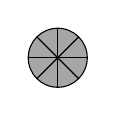
\begin{tikzpicture}[baseline={([yshift={-0.9\ht\strutbox}]current bounding box.north)}]
  %\node at (-1/2,0) {$\ldots\ldots\ldots$};
  \pic  at (0, 0) {circle fraction={8/8}};
\end{tikzpicture}-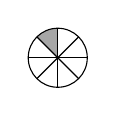
\begin{tikzpicture}[baseline={([yshift={-0.9\ht\strutbox}]current bounding box.north)}]

  %\node at (-1/2,0) {$\ldots\ldots\ldots$};
  \pic  at (0, 0) {circle fraction={1/8}};
\end{tikzpicture}=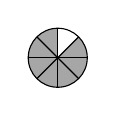
\begin{tikzpicture}[baseline={([yshift={-0.9\ht\strutbox}]current bounding box.north)}]

  %\node at (-1/2,0) {$\ldots\ldots\ldots$};
  \pic  at (0, 0) {circle fraction={7/8}};
\end{tikzpicture}}
\end{center}
}
{1}
\end{resolu}

\begin{exo}
{Que reste-t-il de l'entier 1 si l'on enlève...~?
Représente graphiquement la fraction à l'aide d'un cercle ou d'un rectangle, puis donne la fraction restante.

\begin{tasks}[after-skip=-0.5em](6)
\task $\dfrac{1}{3}$
\task $\dfrac{2}{5}$
\task $\dfrac{3}{8}$
\task $\dfrac{1}{2}$
\task $\dfrac{3}{4}$
\task $\dfrac{2}{7}$
\end{tasks}}
{1}
\end{exo}

\begin{exo}
{Que reste-t-il de l'entier 1 si l'on enlève...~?
Donne la fraction restante.

\begin{tasks}[after-skip=-0.5em](6)
\task $\dfrac{2}{4}$
\task $\dfrac{7}{16}$
\task $\dfrac{9}{21}$
\task $\dfrac{14}{15}$
\task $\dfrac{21}{40}$
\task $\dfrac{11}{30}$
\end{tasks}}
{1}
\end{exo}

\begin{exo}
{Que reste-t-il de l'entier 1 si l'on enlève...~?
Donne la fraction restante.

\begin{tasks}[after-skip=-0.5em](6)
\task $\dfrac{50}{60}$
\task $\dfrac{13}{34}$
\task $\dfrac{25}{67}$
\task $\dfrac{45}{78}$
\task $\dfrac{100}{1000}$
\task $\dfrac{130}{200}$
\end{tasks}}
{1}
\end{exo}
\begin{resolu}{Addition et soustraction de fractions de dénominateurs différents  1/2}{Calcule et donne le résultat sous la forme d'une fraction irréductible ou d'un entier. 

\begin{tasks}
\task \begin{expli}
		\dfrac{1}{2}+\dfrac{1}{4}&=\dfrac{1\cdot 2}{2\cdot 2}+\dfrac{1}{4}& \text{Le }\operatorname{ppmc}(2;4)=4, \text{ donc on amplifie}\\
		      &&\text{par 2 la première fraction pour}\\	
		      &=\dfrac{2}{4}+\dfrac{1}{4}&\text{ avoir des dénominateurs égaux.}\\
		      &&\text{On additionne les fractions}\\
		      &=\dfrac{3}{4}&\text{comme vu précédemment.}\\

		      &&\text{On donne le résultat sous la forme}\\
				&&\text{d'un entier ou d'une fraction irréductible.}
\end{expli}
\task \begin{expli}
		\dfrac{1}{3}-\dfrac{1}{12}&=\dfrac{1\cdot 4}{3\cdot 4}-\dfrac{1}{12}& \text{Le }\operatorname{ppmc}(3;12)=12, \text{ donc on amplifie}\\
		      &&\text{par 4 la première fraction pour}\\	
		      &=\dfrac{4}{12}-\dfrac{1}{12}&\text{ avoir des dénominateurs égaux.}\\
		      &&\text{On soustrait les fractions}\\
		      &=\dfrac{3}{12}&\text{comme vu précédemment.}\\

		      &&\text{On donne le résultat sous la forme}\\
		      &=\dfrac{1}{4}&\text{d'un entier ou d'une fraction irréductible.}
\end{expli}
\end{tasks}}
{1}
\end{resolu}

\begin{exop}
{Pour chacun des calcules suivants:
	\begin{enumerate}
    \item[1)] \text{Trouve le ppcm des deux dénominateurs.}
    \item[2)] \text{Complète les pointillés.}
    \item[3)] {\text Calcule et donne le résultat sous la forme d'une fraction irréductible ou d'un entier.}
\end{enumerate}
\vspace{5pt}

\begin{tasks}
	\task \[\dfrac{9}{4}+\dfrac{5}{12}=\dfrac{9\cdot\ldots\ldots}{4\cdot\ldots\ldots}+\dfrac{5}{12}=\dfrac{\ldots\ldots}{\ldots\ldots}\]
		\vspace{1pt}

		car $\operatorname{ppmc}(4;12)=\ldots\ldots$. 
	\task \[\dfrac{8}{5}-\dfrac{16}{10}=\dfrac{8\cdot\ldots\ldots}{5\cdot\ldots\ldots}-\dfrac{16}{10}=\dfrac{\ldots\ldots}{\ldots\ldots}\]
		\vspace{1pt}

	car $\operatorname{ppmc}(5;10)=\ldots\ldots$.
	\task \[\dfrac{5}{6}+\dfrac{5}{12}=\dfrac{5\cdot\ldots\ldots}{6\cdot\ldots\ldots}+\dfrac{5}{12}=\dfrac{\ldots\ldots}{\ldots\ldots}\]
		\vspace{1pt}

		car $\operatorname{ppmc}(6;12)=\ldots\ldots$.
	\task \[\dfrac{2}{3}-\dfrac{1}{18}=\dfrac{2\cdot\ldots\ldots}{3\cdot\ldots\ldots}-\dfrac{1}{18}=\dfrac{\ldots\ldots}{\ldots\ldots}\]
		\vspace{1pt}

	car $\operatorname{ppmc}(3;18)=\ldots\ldots$.
\end{tasks}}
{1}
\end{exop}

\begin{exo}
{Calcule et donne le résultat sous la forme d'une fraction irréductible ou d'un entier. 
\begin{tasks}(3)
\task $\dfrac{3}{5}+\dfrac{8}{10}=$
\task $\dfrac{2}{7}+\dfrac{1}{14}=$
\task $\dfrac{4}{15}+\dfrac{3}{5}=$
\task $\dfrac{5}{8}+\dfrac{1}{4}=$
\task $\dfrac{5}{6}+\dfrac{7}{12}=$
\task $\dfrac{2}{3}+\dfrac{3}{6}=$
\task $\dfrac{7}{15}+\dfrac{5}{3}=$
\task $\dfrac{3}{8}+\dfrac{5}{16}=$
\end{tasks}
}{1}
\end{exo}



\begin{exo}
{Calcule et donne le résultat sous la forme d'une fraction irréductible ou d'un entier. 

\begin{tasks}(3)
 \task $\dfrac{5}{6}+\dfrac{5}{12}=$
  \task $\dfrac{11}{3}-\dfrac{5}{6}=$
 \task $\dfrac{13}{14}+\dfrac{5}{7}=$
  \task $\dfrac{11}{9}-\dfrac{1}{3}=$  
  \task $\dfrac{3}{25}+\dfrac{2}{5}=$  
  \task $\dfrac{4}{3}-\dfrac{5}{21}=$  
\end{tasks}    
}{1}
\end{exo}

\begin{exo}
{Calcule et donne le résultat sous la forme d'une fraction irréductible ou d'un entier.

\begin{tasks}(3)
\task $\dfrac{1}{2}-\dfrac{1}{4}=$
\task $\dfrac{3}{2}-\dfrac{1}{8}=$
\task $\dfrac{3}{4}-\dfrac{3}{12}=$
\task $\dfrac{3}{6}-\dfrac{1}{2}=$
\task $\dfrac{3}{4}-\dfrac{5}{8}=$
\task $\dfrac{7}{8}-\dfrac{3}{4}=$
\end{tasks}}
{1}
\end{exo}

\begin{exo}
{Calcule et donne le résultat sous la forme d'une fraction irréductible ou d'un entier.

\begin{tasks}(3)
\task $\dfrac{2}{3}-\dfrac{1}{6}=$
\task $\dfrac{9}{10}-\dfrac{2}{5}=$
\task $\dfrac{3}{4}-\dfrac{7}{12}=$
\task $\dfrac{8}{9}-\dfrac{1}{3}=$
\task $\dfrac{7}{6}-\dfrac{5}{12}=$
\task $\dfrac{3}{5}-\dfrac{4}{15}=$
\end{tasks}}
{1}
\end{exo}


\begin{resolu}{Addition et soustraction de fractions de dénominateurs différents 2/2}{
Calcule et donne le résultat sous la forme d'une fraction irréductible ou d'un entier. 
\vspace{5pt}

\begin{tasks}
\task \begin{expli}
		\dfrac{11}{8}+\dfrac{5}{6}&=\dfrac{11\cdot 3}{8\cdot 3}+\dfrac{5\cdot 4}{6\cdot 4}& \text{Le }\operatorname{ppmc}(8;6)=24, \text{ on amplifie par 3}\\
		      &&\text{la première fraction et par 4 la deuxième}\\	
		      &=\dfrac{33}{24}+\dfrac{20}{24}&\text{pour avoir des dénominateurs égaux.}\\
		      &&\text{On additionne les fractions}\\
		      &=\dfrac{53}{24}&\text{comme vu précédemment.}\\

		      &&\text{On donne le résultat sous la forme}\\
		      &&\text{d'un entier ou d'une fraction irréductible.}
\end{expli}
\task \begin{expli}
		\dfrac{5}{9}-\dfrac{1}{4}&=\dfrac{5\cdot 4}{9\cdot 4}-\dfrac{1\cdot 9}{4\cdot 9}& \text{Le }\operatorname{ppmc}(9;4)=36, \text{ on amplifie par 4}\\
		      &&\text{la première fraction et par 9 la deuxiÚme}\\	
		      &=\dfrac{20}{36}-\dfrac{9}{36}&\text{pour avoir des dénominateurs égaux.}\\
		      &&\text{On soustrait les fractions}\\
		      &=\dfrac{11}{36}&\text{comme vu précédemment.}\\

		      &&\text{On donne le résultat sous la forme}\\
		      &&\text{d'un entier ou d'une fraction irréductible.}
\end{expli}
\end{tasks}}
{1}
\end{resolu}

\begin{exop}
{Pour chacun des calculs suivants:
	\begin{enumerate}
    \item[1)] \text{Trouve le ppcm des deux dénominateurs.}
    \item[2)] \text{Complète les pointillés.}
    \item[3)] {\text Calcule et donne le résultat sous la forme d'une fraction irréductible ou
    d'un entier.}
\end{enumerate}
\vspace{3pt}

\begin{tasks}
	\task \[\dfrac{5}{9}+\dfrac{7}{4}=\dfrac{5\cdot\ldots\ldots}{9\cdot\ldots\ldots}+\dfrac{7\cdot \ldots\ldots}{4\cdot \ldots\ldots}=\dfrac{\ldots\ldots}{\ldots\ldots}\]
		\vspace{3pt}

	car $\operatorname{ppmc}(9;4)=\ldots\ldots$.
	\task \[\dfrac{5}{3}-\dfrac{5}{4}=\dfrac{5\cdot\ldots\ldots}{3\cdot\ldots\ldots}-\dfrac{5\cdot \ldots\ldots}{4\cdot \ldots\ldots}=\dfrac{\ldots\ldots}{\ldots\ldots}\]
		\vspace{3pt}

	car $\operatorname{ppmc}(3;4)=\ldots\ldots$.
	\task \[\dfrac{2}{3}+\dfrac{8}{5}=\dfrac{2\cdot\ldots\ldots}{3\cdot\ldots\ldots}+\dfrac{8\cdot \ldots\ldots}{5\cdot \ldots\ldots}=\dfrac{\ldots\ldots}{\ldots\ldots}\]
		\vspace{3pt}

	car $\operatorname{ppmc}(3;5)=\ldots\ldots$.
	\task \[\dfrac{5}{10}-\dfrac{2}{15}=\dfrac{5\cdot\ldots\ldots}{10\cdot\ldots\ldots}-\dfrac{2\cdot \ldots\ldots}{15\cdot \ldots\ldots}=\dfrac{\ldots\ldots}{\ldots\ldots}\]
		\vspace{3pt}

	car $\operatorname{ppmc}(10;15)=\ldots\ldots$.
\end{tasks}}
{1}
\end{exop}



\begin{exo}
{Calcule et donne le résultat sous la forme d'une fraction irréductible ou d'un entier.
\begin{tasks}(3)
\task $\dfrac{2}{3}+\dfrac{6}{5}=$
\task $\dfrac{3}{2}-\dfrac{1}{3}=$
\task $\dfrac{7}{3}-\dfrac{3}{2}=$
\task $\dfrac{13}{52}-\dfrac{1}{20}=$
\task $\dfrac{5}{9}+\dfrac{2}{18}=$
\task $\dfrac{5}{6}+\dfrac{2}{8}=$
\end{tasks}    
}{1}
\end{exo}

\begin{exo}
{Calcule et donne le résultat sous la forme d'une fraction irréductible ou d'un entier.
\begin{tasks}(3)
\task $\dfrac{3}{4}+\dfrac{5}{7}=$
\task $\dfrac{13}{14}-\dfrac{1}{4}=$
\task $\dfrac{5}{11}-\dfrac{2}{33}=$
\task $\dfrac{6}{12}+\dfrac{3}{36}=$
\task $\dfrac{3}{9}+\dfrac{2}{18}=$
\task $\dfrac{6}{24}+\dfrac{3}{4}=$
\end{tasks}    
}{1}
\end{exo}


\begin{resolu}{Fraction et entier}{
Calcule et donne le résultat sous la forme d'une fraction irréductible ou d'un entier. 
\vspace{5pt}

\begin{tasks}
\task 
\begin{expli}
	1+\dfrac{1}{4}&=\dfrac{1}{1}+\dfrac{1}{4}& \text{On passe en écriture fractionnaire.}\\
		      &&\text{On amplifie pour avoir des}\\	
		      &=\dfrac{1\cdot 4}{1 \cdot 4}+\dfrac{1}{4}&\text{dénominateurs égaux.}\\
		      &&\text{On additionne les fractions}\\
		      &=\dfrac{4}{4}+\dfrac{1}{4}&\text{comme vu prcédemment.}\\

		      &&\text{On donne le résultat sous la forme}\\
				&=\dfrac{5}{4}&\text{d'un entier ou d'une fraction irréductible.}
\end{expli}

\task \begin{expli}
	2-\dfrac{1}{6}&=\dfrac{2}{1}-\dfrac{1}{6}& \text{On passe en écriture fractionnaire.}\\
		      &&\text{On amplifie pour avoir des}\\	
		      &=\dfrac{2\cdot 6}{1 \cdot 6}+\dfrac{1}{6}&\text{dénominateurs égaux.}\\
		      &&\text{On soustrait les fractions}\\
		      &=\dfrac{12}{6}-\dfrac{1}{6}&\text{comme vu précédemment.}\\

				&&\text{On donne le résultat sous la forme}\\
				&=\dfrac{11}{6}&\text{d'un entier ou d'une fraction irréductible.}
\end{expli}
\end{tasks}}
{1}
\end{resolu}

\vfill

\begin{exo}
{Complète les pointillés, puis calcule et donne le résultat sous la forme d'une fraction irréductible ou d'un entier. 
\begin{tasks}(2)
\task $1+\dfrac{2}{6}= \dfrac{1\cdot\ldots}{1\cdot\ldots}+ \dfrac{2}{6}= $ 
\task $2+\dfrac{1}{3}=\dfrac{2\cdot\ldots}{1\cdot\ldots}+ \dfrac{1}{3}=$ 
\task $\dfrac{16}{3}+3=\dfrac{16}{3}+\dfrac{3\cdot\ldots}{1\cdot\ldots}=$
\task $\dfrac{3}{4}+2=\dfrac{3}{4}+\dfrac{2\cdot\ldots}{1\cdot\ldots}=$
\end{tasks}
}{1}
\end{exo}

\vfill

\begin{exo}
{Complète les pointillés, puis calcule et donne le résultat sous la forme d'une fraction irréductible ou d'un entier. 
\begin{tasks}(2)
\medskip\task $1-\dfrac{2}{6}= \dfrac{1\cdot\ldots}{1\cdot\ldots}- \dfrac{2}{6}=$ 
\medskip \task $2-\dfrac{1}{3}=\dfrac{2\cdot\ldots}{1\cdot\ldots}- \dfrac{1}{3}=$ 
\medskip \task $\dfrac{16}{3}-3= \dfrac{16}{3}-\dfrac{3\cdot\ldots}{1\cdot\ldots}=$ 
\medskip \task $\dfrac{13}{4}-2=\dfrac{13}{4}-\dfrac{2\cdot\ldots}{1\cdot\ldots}=$
\end{tasks}
}{1}
\end{exo}

\vfill

\newpage
\begin{exo}
{Calcule et donne le résultat sous la forme d'une fraction irréductible ou d'un entier. 
\begin{tasks}(3)
\task $4-\dfrac{3}{2}= $ 
 \task $2+\dfrac{1}{4}=$ 
 \task $\dfrac{9}{4}-1=$
 \task $4+\dfrac{5}{7}=$
 \task $\dfrac{16}{3}-2=$
 \task $2+\dfrac{3}{4}=$ 
\end{tasks}
}{1}
\end{exo}

\begin{exop}
{Complète les pointillés  par un nombre entier:	
\begin{tasks}(3)
\task $\dfrac{4}{6}+\dfrac{\ldots\ldots\ldots}{6}=1$
\task $\dfrac{2}{3}+\dfrac{\ldots\ldots\ldots}{3}=1$

\task $\dfrac{4}{9}+\dfrac{\ldots\ldots\ldots}{\ldots\ldots\ldots}=1$
\task $\dfrac{7}{8}+\dfrac{\ldots\ldots\ldots}{\ldots\ldots\ldots}=1$
\task $\dfrac{4}{5}+\dfrac{\ldots\ldots\ldots}{5}=1$
\task $\dfrac{81}{83}+\dfrac{\ldots\ldots\ldots}{\ldots\ldots\ldots}=1$
\end{tasks}
}{1}
\end{exop}

\begin{resolu}{Fractions et décimaux}{Calcule et donne le résultat sous la forme d'une fraction irréductible ou d'un entier. 
		\vspace{5pt}

\begin{tasks}
\task \begin{expli}
		\dfrac{7}{5}+7,5&=\dfrac{7}{5}+\dfrac{75}{10}& \text{On passe en écriture fractionnaire.}\\
		      &&\text{On amplifie pour avoir des}\\	
		      &=\dfrac{7\cdot 2}{5\cdot 2}+\dfrac{75}{10}&\text{dénominateurs égaux.}\\
		      &&\text{On additionne les fractions}\\
		      &=\dfrac{14}{10}+\dfrac{75}{10}&\text{comme vu précédemment.}\\

		      &&\text{On donne le résultat sous la forme}\\
				&=\dfrac{89}{10}&\text{d'un entier ou d'une fraction irréductible.}
\end{expli}

\task \begin{expli}
		\dfrac{11}{8}+1,25&=\dfrac{11}{8}+\dfrac{125}{100}& \text{On passe en écriture fractionnaire.}\\
		      &&\text{On amplifie pour avoir des}\\	
		      &=\dfrac{11\cdot 25}{8 \cdot 25}+\dfrac{125\cdot 2}{100\cdot 2}&\text{dénominateurs égaux.}\\
		      &&\text{On additionne les fractions}\\
		      &=\dfrac{275}{200}+\dfrac{250}{200}&\text{comme vu précédemment.}\\
		      &&\text{On donne le résultat sous }\\
		      &=\dfrac{525}{200}&\text{la forme d'un entier ou}\\
		      &&\text{d'une fraction irréductible.}\\
				&=\dfrac{21}{8}&
\end{expli}
\end{tasks}}
{1}
\end{resolu}

\begin{exop}
{Pour chacun des calculs suivants:
	\begin{enumerate}
    \item[1)] Transforme le nombre décimal en une fraction décimale.
    \item[2)] Trouve le ppmc des deux dénominateurs.
    \item[3)] Complète les pointillés.
    \item[4)] Calcule et donne le résultat sous la forme d'une fraction irréductible ou d'un entier.
\end{enumerate}
\vspace{1pt}

\begin{tasks}
	\task \[\dfrac{13}{6}-1,5=\dfrac{13}{6}-\dfrac{\ldots\ldots}{\ldots\ldots}=\dfrac{13\cdot \ldots\ldots}{6\cdot \ldots\ldots}-\dfrac{\ldots\ldots}{\ldots\ldots}=\dfrac{\ldots\ldots}{\ldots\ldots}\]
\vspace{1pt}

		car $\operatorname{ppmc}(6;\ldots\ldots)=\ldots\ldots$.

	\task \[1,2+\dfrac{3}{5}=\dfrac{\ldots\ldots}{\ldots\ldots}+\dfrac{3}{5}=\dfrac{\ldots\ldots}{\ldots\ldots}+\dfrac{3\cdot \ldots\ldots}{5\cdot \ldots\ldots}=\dfrac{\ldots\ldots}{\ldots\ldots}\]
\vspace{1pt}

		car $\operatorname{ppmc}(\ldots\ldots;5)=\ldots\ldots$.
	\task \[0,5+1,75=\dfrac{\ldots\ldots}{\ldots\ldots}+\dfrac{\ldots\ldots}{\ldots\ldots}=\dfrac{\ldots\ldots}{\ldots\ldots}+\dfrac{\ldots\ldots}{\ldots\ldots}=\dfrac{\ldots\ldots}{\ldots\ldots}\]
\vspace{1pt}

		car $\operatorname{ppmc}(\ldots\ldots;\ldots\ldots)=\ldots\ldots$.
\end{tasks}}
{1}
\end{exop}



\begin{exo}
 {Calcule et donne le résultat sous la forme d'une fraction irréductible ou d'un entier.
	 \begin{tasks}(2)
\task $\dfrac{2}{3}+0,5=$
\task $\dfrac{13}{5}-1,5=$
\task $4,5-\dfrac{1}{4}=$
\task $7,35-\dfrac{3}{5}=$
\end{tasks}}
{1}
\end{exo}

\begin{resolu}{Fractions et périodiques}{Voici une liste de fractions utiles:
		\begin{tasks}(2)
    \task $\dfrac{1}{3}=0,\overline{3} $
    \task $\dfrac{2}{3}=0,\overline{6} $
    \task $\dfrac{1}{9}=0,\overline{1}$
    \task $\dfrac{1}{7}=0,\overline{142857}$
\end{tasks}

Calcule et donne le résultat sous la forme d'une fraction irréductible ou d'un entier. 

\begin{tasks}(2)
    \task $\dfrac{1}{2}+0,\overline{3}=\dfrac{1}{2}+ \dfrac{1}{3}=\dfrac{5}{6}$
   \task $0,\overline{6}+\dfrac{1}{3}=\dfrac{2}{3}+\dfrac{1}{3}=\dfrac{3}{3}=1$
\end{tasks}}
{1}
\end{resolu}

\vfill

\begin{exo}
{Calcule et donne le résultat sous la forme d'une fraction irréductible ou d'un entier.

	\begin{tasks}(2)
\task $\dfrac{8}{9}-0,\overline{6}=$
\task$\dfrac{1}{2}-0,\overline{3}=$
\task $\dfrac{4}{9}+0,\overline{3}=$
\task $\dfrac{1}{4}+0,\overline{6}=$
\end{tasks}}
{1}
\end{exo}

\vfill

\begin{exo}
 {Calcule et donne le résultat sous la forme d'une fraction irréductible ou d'un entier.

	 \begin{tasks}(2)
\task $\dfrac{5}{8}+17,05=$
\task$0,5-0,\overline{3}=$
\task $ 3,45+0,\overline{3}=$
\task $\dfrac{1}{8}+3,\overline{6}=$
\end{tasks}
}
{2}
\end{exo}


\vfill

\newpage


\vfill

\begin{exo}
 {Calcule et donne le résultat sous la forme d'une fraction irréductible ou d'un entier.
\begin{tasks}(3)
 \task  $\dfrac{5}{3}+2-\dfrac{3}{4}=$
 \task  $\dfrac{7}{8}+2,5+\dfrac{1}{16}=$
 \task $3,6-\dfrac{1}{3}=$
 \task  $0,025+2-\dfrac{1}{3}=$
 \task  $\dfrac{2}{3}+\dfrac{3}{4}-1=$
 \task $0,6-\dfrac{1}{3}=$
\end{tasks}
}{1}
\end{exo}


\begin{exo}
{Calcule et donne le résultat sous la forme d'une fraction irréductible ou d'un entier.
	\begin{tasks}(2)
\task $\dfrac{1}{2}+\dfrac{5}{12}+0,\overline{3}=$
\task $30,05+\dfrac{2}{5}=$
\task $\dfrac{4}{7}-0,\overline{3}=$
\task $0,05+\dfrac{1}{4}+0,\overline{6}=$
\task $5+\dfrac{2}{11}=$
\task $9,2-1,\overline{3}=\phantom{\dfrac{1}{5}}$
\end{tasks}}
{2}
\end{exo}

\newpage

\begin{exo}
{Complètes les pointillés par un entier.

\begin{tasks}(2)
\task  $\dfrac{4}{5}+\dfrac{\ldots}{\ldots}=\dfrac{21}{20}$
\task $\dfrac{2}{3}+3=\dfrac{\ldots}{\ldots}$
\task $1,\overline{3}-\dfrac{\ldots}{\ldots}=0,5$
\task  $\dfrac{13}{52}-\dfrac{8}{20}=\dfrac{\ldots}{\ldots}$
\task  $1,\overline{6}+0,\overline{3}=\dfrac{\ldots}{\ldots}\phantom{\dfrac{1}{2}}$
\task $\dfrac{6}{3}-\dfrac{\ldots}{\ldots}=\dfrac{7}{6}$
\end{tasks}
}
{2}
\end{exo}

\begin{exof}{NO118}{40}{1}
\end{exof}
\begin{exof}{NO123}{40}{1}
\end{exof}
\begin{exof}{NO124}{41}{1}
\end{exof}
\begin{exof}{NO125}{41}{1}
\end{exof}


\begin{exo}
{J'ai mangé un quart, puis deux tiers d'un gâteau. 
\begin{tasks}[after-item-skip = 0.2em]
    \task Quelle fraction du gâteau ai-je mangé~?
    \task Quelle fraction du gâteau reste-t-il~?
\end{tasks}}
{1}
\end{exo}

\begin{exo}
{\vspace{0.5em}

	Marc a dépensé $\dfrac{1}{4}$ de son argent de poche pour s'acheter une BD et $\dfrac{2}{3}$ pour acheter un cadeau à sa soeur.


\begin{tasks}[after-item-skip = 0.2em]
    \task Quelle fraction de son argent a-t-il dépensé~?
    \task Quelle fraction lui reste-t-t-il~?
\end{tasks}}
{1}
\end{exo}

\begin{exo}
	{\vspace{0.5em}

		J'ai passé le $\dfrac{3}{7}$ de mes vacances en Italie et les $\dfrac{2}{14}$ chez mes grands-parents. Le reste, je les passe tranquillement chez moi.

		\begin{tasks}[after-item-skip = 0.2em]
    \task Quelle fraction de mes vacances ai-je passé hors de chez moi~?
    \task Quelle fraction de mes vacances suis-je resté chez moi~?
\end{tasks}}
{1}
\end{exo}


\begin{exol}{NO119}{39}{1}
\end{exol}
\begin{exol}{NO136}{43}{1}
\end{exol}
\begin{exol}{NO139}{43}{1}
\end{exol}



\end{document}